\documentclass[conference]{IEEEtran}
\oddsidemargin  0pt     %   Left margin on odd-numbered pages.
\evensidemargin 0pt     %   Left margin on even-numbered pages.
\marginparwidth 40pt    %   Width of marginal notes.
\marginparsep 10pt      % Horizontal space between outer margin and
                        % marginal note
\topmargin 0pt          % Nominal distance from top of page to top of
                        %    box containing running head.
\headsep 10pt           %    Space between running head and text.
\textheight 8.4in       % Height of text(including footnotes and figures,
                        % excluding running head and foot).
\textwidth 6.6in        % Width of text line.

\setlength{\floatsep}{2mm}
\setlength{\textfloatsep}{2mm}
\usepackage{secdot}
\usepackage{setspace}
\usepackage{hyperref}
\usepackage{latexsym}
\usepackage{amsfonts}
\usepackage{amsmath}
\usepackage{amsthm}
\usepackage{amssymb}
\usepackage{color}
\usepackage{graphicx}
\usepackage{subfigure}
\usepackage{algorithm}
\usepackage{algorithmicx}
\usepackage{algpseudocode}
\usepackage{epstopdf}
\usepackage{flushend}

\hypersetup{
    bookmarks=false,         % show bookmarks bar?
    unicode=false,          % non-Latin characters in Acrobat’s bookmarks
    pdftoolbar=true,        % show Acrobat’s toolbar?
    pdfmenubar=true,        % show Acrobat’s menu?
    pdffitwindow=true,      % page fit to window when opened
    pdftitle={Parallel Algorithms for Graph Optimization using Tree Decompositions},%title
    pdfauthor={Blair Sullivan, Dinesh Weerapurage, Chris Gro\"er},     % author
    pdfsubject={Subject},   % subject of the document
    pdfcreator={Creator},   % creator of the document
    pdfproducer={Producer}, % producer of the document
    pdfkeywords={graph algorithms, parallel computing, tree decomposition, dynamic
      programming, weighted independent set, discrete optimization}, % list of keywords
    pdfnewwindow=true,      % links in new window
    colorlinks=true,       % false: boxed links; true: colored links
    linkcolor=black,          % color of internal links
    citecolor=black,        % color of links to bibliography
    filecolor=black,      % color of file links
    urlcolor=black           % color of external links
}

 % My commands
\renewcommand{\thefootnote}{\fnsymbol{footnote}}
\newcommand{\p}{\phantom}
\newcommand{\red}[1]{\textcolor{black}{#1}}
\widowpenalty=12000
\clubpenalty=12000
\hyphenation{op-tical net-works semi-conduc-tor}
\begin{document}
\title{Parallel Algorithms for Graph Optimization using Tree Decompositions}
% author names and affiliations
% use a multiple column layout for up to three different
% affiliations
\author{\IEEEauthorblockN{Blair D. Sullivan}
\IEEEauthorblockA{Oak Ridge National Laboratory \\
P.O. Box 2008 MS6015 \\
Oak Ridge, TN 37831-6015 \\
sullivanb@ornl.gov}
\and
\IEEEauthorblockN{Dinesh Weerapurage}
\IEEEauthorblockA{Link Analytics\\
1050 Crown Pointe Pkwy, Ste 1580\\
Atlanta, GA 30338\\
dinesh.weerapurage@linkanalytics.com}
\and
\IEEEauthorblockN{Chris Gro\"er}
\IEEEauthorblockA{Link Analytics \\
1050 Crown Pointe Pkwy, Ste 1580\\
Atlanta, GA 30338\\
chris.groer@linkanalytics.com}}
\maketitle
\footnote{The submitted manuscript has been authored by a contractor of the U.S. Government under
Contract No. DE-AC05-00OR22725. Accordingly, the U.S. Government retains a non-exclusive,
royalty-free license to publish or reproduce the published form of this contribution, or
allow others to do so, for U.S. Government purposes.}
\begin{abstract}
Although many NP-hard graph optimization problems can be solved in
polynomial time on graphs of bounded tree-width, the adoption of these
techniques into mainstream scientific computation has been limited due
to the high memory requirements of the dynamic programming tables
and excessive runtimes of sequential implementations.  This work
addresses both challenges by proposing a set of new parallel
algorithms for all steps of a tree decomposition-based approach to
solve the maximum weighted independent set problem.  A hybrid OpenMP/MPI
implementation includes a highly scalable parallel dynamic programming
algorithm leveraging the MADNESS task-based runtime, and computational
results demonstrate scaling. This work enables a significant expansion
of the scale of graphs on which exact solutions to maximum weighted
independent set can be obtained, and forms a framework for solving
additional graph optimization problems with similar techniques.
\\
\emph{Keywords:} {graph algorithms, dynamic programming, parallel programming,
  independent set, tree decomposition, }
\end{abstract}
\IEEEpeerreviewmaketitle

\section{Introduction}

Discrete optimization problems on graphs are
notoriously difficult to parallelize and finding exact solutions to
such optimization problems is often severely limited by the size of the instance.  Algorithms
based on tree decompositions provide a tantalizing possibility, since
the complexity of many NP-hard optimization problems
is transformed to become polynomial in the number of vertices in the
graph (and exponential in the decomposition's width). 
% bds - having trouble with apostrophe here
% CSGCSG - deleted quotes

Tree decompositions were introduced by Robertson and Seymour in 1984
\cite{RobertsonSeymour1984} as tools in the proof of the Graph Minors Theorem.
Each decomposition has an associated measure of width, and the minimal achievable width
for a graph is its treewidth. This can be thought of as a measure of how ``tree-like'' the graph is.
The computational community became interested in tree decompositions after it was
shown that numerous NP-hard graph problems can be solved in polynomial time
on graphs with bounded treewidth \cite{Courcelle1990Rewriting}.

However, nearly all the work assessing the viability of parallel approaches has been
purely theoretical in nature.
One potential reason for the lack of parallel approaches is that
the memory requirements for tree decomposition-based
dynamic programming can be staggering, even for graphs with very few nodes and edges.
For example, a good heuristic produces a decomposition with width 313 for the
DIMACS challenge graph \emph{1dc.512}. \cite{DIMACS}  The largest bag in this decomposition could
require roughly $10^{14}$ bytes of memory for its dynamic programming table (if almost all subsets were independent).
%BDS - reworded below sentence; added clarification on memory usage above.
We are aware of no other implementations of parallel algorithms for either the construction of a tree decomposition or the
subsequent dynamic programming.  
Here we present the first
serious effort to address the various computational issues by
applying high performance computing (HPC) to this area.

There is a potential for parallelism inherent to tree decomposition-based algorithms: (i) the dynamic programming computation at each node in the tree decomposition requires only partial information
about the graph, and (ii) the dynamic programming tables
for large sets of tree nodes can be computed independently of
one another.
While the dynamic programming tables for the leaf nodes in the tree decomposition
can be computed simultaneously, the computation as a whole is difficult to
parallelize. One might think that one could proceed up the levels of the tree in a
bulk-synchronous fashion. However, this is a poor strategy for a number of reasons.
First, the amount of work at each tree node is $O(w^{\log w})$ \cite{wilfcomplexity}.
Since the size of the bags in the tree decomposition can vary quite a bit,
this growth can lead to wide variation in the amount of time required to process a tree node.
Second, the tree itself can be very unbalanced (see Figure \ref{fig:unbalanced_tree}) and since we can't process a tree node
until all nodes below it are processed, this leads to a very asynchronous workload
that is very difficult to load balance.
These features of the tree and the related dynamic programming
force one to adopt a non-traditional approach when designing a parallel
algorithm.
Our work leverages the task-based framework offered
by MADNESS (Multiresolution Adaptive Numerical
Environment for Scientific Simulation) ~\cite{Thorntonintroducing} in order to handle the work distribution,
load balancing, and asynchronous nature of the dynamic
programming. For graphs with large size (which we measure by the number of vertices) and low treewidth, the results are compelling, and we achieve near linear speedups relative to a serial implementation. 

% CSG inserting PR124_TD.pdf here
\begin{figure*}[!th]
\begin{center}
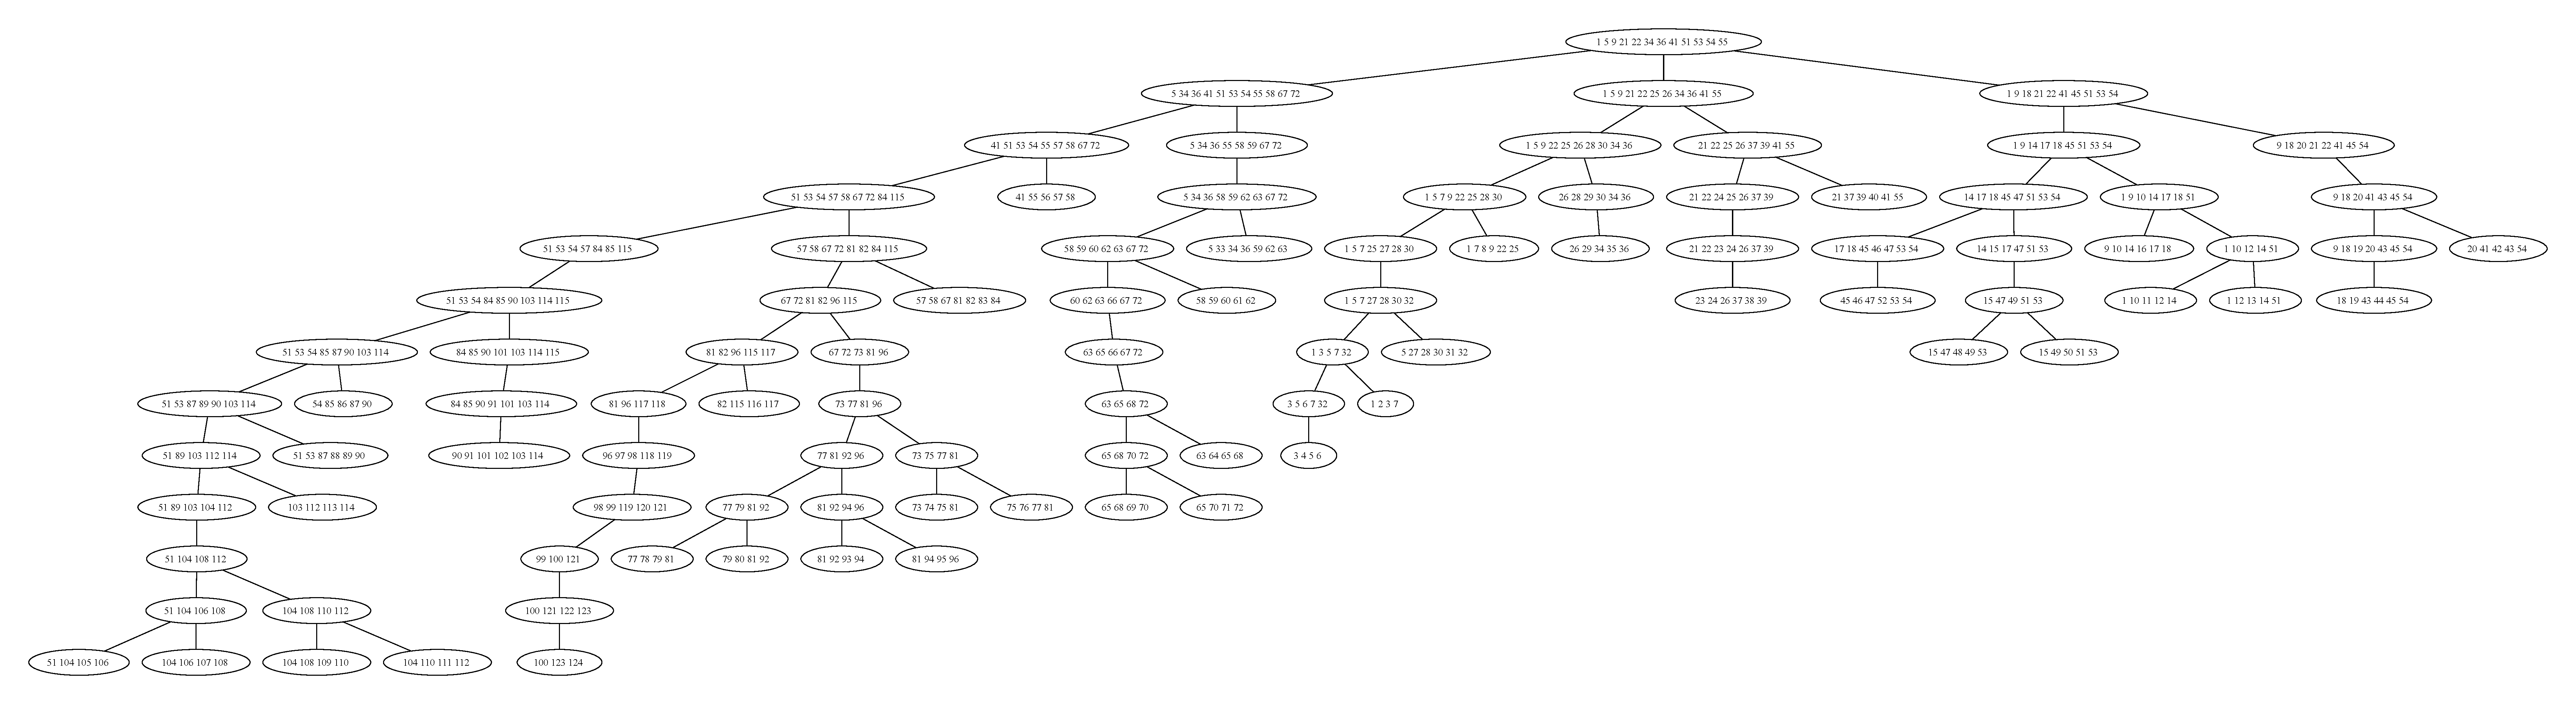
\includegraphics[height=1.5in]{figures/pr124_TD.pdf}
\caption{A tree decomposition of a 124-node graph that exhibits a very unbalanced structure that makes
a layer-by-layer dynamic programming approach very inefficient}
\label{fig:unbalanced_tree}
\end{center}
\end{figure*}


% CSGCSG commenting out since Gurobi experimentw as a failure...
%These new algorithmic enhancements and improvements in implementation efficiency enable us to exactly 
%solve optimization problems on networks that are several orders of magnitude larger (in terms of the number of
%nodes/edges) than attainable with other methods from the literature.

The algorithms described in this paper have been implemented as part of the
open source INDDGO\footnotemark software package~\cite{inddgo}.
\footnotetext{Integrated Network Decompositions and Dynamic programming for Graph Optimization}

%BDS add quote about sextillion processors, reference to cliquewidth paper where analysis is of graphs with 300 nodes, max tw for 'feasibility' quote from prior slides/proposal. Emphasize novelty of work.

%Solving optimization problems on graphs of bounded treewidth relies on finding %a low-width tree decomposition
%(since the complexity is typically exponential in the width), then running a dy%namic programming algorithm
%which computes and merges tables of partial solutions at each tree node. The pr%oblem of finding an optimal (minimum
%width) tree decomposition is itself $\cal NP$-hard~\cite{SeymourThomas1994}, an%d existing algorithms offer either a guarantee on the quality of the approximat%ion at the expense of computational feasibility
%(e.g. Bodlaender \cite{Bodlaender1996} was shown in \cite{Rohrig1998} to be inf%easible even for graphs of width four),
%or provide no guarantees but reasonable running times. We work with an approach% from the latter category,
%based on elimination orderings and a construction by Gavril~\cite{Gavril1974int%ersection}. The dynamic programming
%step...%BDS - continue here. NOT DONE NOT DONE

\section{Background}

\subsection{Definitions and terminology}
Formally, a {\em graph} $G=(V,E)$ is a set of vertices $V$ and a set of edges $E$ formed by unordered pairs of vertices. All graphs in this paper are assumed to be finite, simple and undirected. We also assume the graphs under consideration are {\em connected}, since otherwise, the techniques being discussed here can be applied to find solutions for each connected component, which can then be easily combined into a solution for the entire graph.

For a vertex $v \in V$, let $N(v) = \{u\,:\,(u,v) \in E\}$ be the
{\em neighbors} of $v$. We say $H = (W,F)$ is a {\em subgraph} of $G = (V,E)$, denoted
$H \subseteq G$,  if both $W \subseteq V$ and $F \subseteq E$.
An  {\em induced subgraph} is one that satisfies $(x,y) \in F$ for every pair $x,y \in W$ such that $(x,y)\in E$. We denote the induced subgraph of $G$ with
vertices $X \subseteq V$ as $G[X]$.

The last graph-related definition we need is of {\em chordal} graphs ---
those where every cycle with more than three vertices has an edge connecting two non-consecutive
vertices~\cite{Gavril1974intersection}.

A {\em tree decomposition} of a
graph $G = (V,E)$ is a pair $(X,T)$, where $X = \{X_1, \ldots, X_n\}$
is a collection of subsets of $V$ and $T = (I,F)$ is a tree (acyclic graph) with $I =
\{1,\ldots,n\}$, satisfying three conditions:
\begin{enumerate}
\item $\cup_{i\in I} X_i$ is equal to the vertex set $V$
  ($i \in I$),
\item for every edge $uv$ in $G$, $\{u,v\} \subseteq X_i$ for some $i
  \in I$, and
\item for every $v \in V$, if $X_i$ and $X_j$ contain $v$ for some
  $i,j \in I$, then $X_k$ also contains $v$ for all $k$ on the
  (unique) path in $T$ connecting $i$ and $j$. In other words, the set
  of nodes whose associated subsets contain $v$ form a connected subtree of
  $T$.
\end{enumerate}

Note that we will use the term {\em vertex} to refer to elements of $V$ and {\em node}
to to refer to elements of $I$ to avoid confusion. The subsets $X_i$ are often referred
to as \emph{bags} of vertices. The {\em width} of a tree decomposition
$(X, (I,F))$ is the maximum over $i \in I$ of
% CSGCSG - above was 1 \in I??
$|X_i|-1$, and the {\em treewidth} of a graph $G$, denoted $\tau(G)$,
is the minimum width over all valid tree decompositions of $G$. An {\em optimal tree
  decomposition} for a graph $G$ is one with width $\tau(G)$.

An important class of graphs of class used in this paper are the {\em
  $k$-trees}, which are defined recursively. In the smallest
case, a clique on $k+1$ vertices is a $k$-tree. Otherwise,  for $n >
k$, a $k$-tree on $n+1$ vertices can be constructed from a
$k$-tree $H$ on $n$ vertices by adding a new vertex $v$ adjacent to
some set of $k$ vertices which form a clique in H. A $k$-tree has
treewidth exactly $k$ (the bags of the optimal tree decomposition are
the cliques of size $k+1$). We call the set of all subgraphs of
$k$-trees the {\em partial $k$-trees}.  It easy to see that any
partial $k$-tree has treewidth at most $k$ (one can derive a valid
tree decomposition of width $k$ from that of the $k$-tree which
contains it). Furthermore, any graph with treewidth at most $k$ is
the subgraph of some $k$-tree~\cite{Leeuwen1990}. Thus the set of all graphs with
treewidth at most $k$ can be generated by finding all $k$-trees and
their subgraphs, leading us to a simple generator for random graphs
of bounded treewidth.

In this paper, randomly generated partial $k$-trees are
denoted with the prefix ``pkt" followed
by the number of nodes, maximum width, and edge density. For example,
pkt.500000.10.80 is a partial $k$-tree generated by keeping 80\% of the
edges from a random $10$-tree on 500,000 nodes. We may write things like
pkt.500000.width.80 to denote a set of graphs that all have 500,000 nodes
and 80\% of the edges of their parent $k$-tree, whose treewidth ($k$) is
being varied.

\subsection{Sequential Algorithms}\label{sec:seq_algorithm}

Before presenting the details of our parallel algorithm and related computational results, we describe the general idea behind a serial algorithm for solving the maximum weighted independent set (MWIS) problem using dynamic programming and discuss the various bottlenecks that one encounters in the serial environment. 
The general process for solving MWIS using tree decompositions to achieve fixed parameter tractability is shown in Figure~\ref{fig:sequential.algorithm}.  
At a high level, after initializing the graph, an elimination ordering is computed and used to
guide triangulation, a process of adding edges to make the graph chordal. 
% CSGCSG removing this - we don't have these anymore
% (line~\ref{} \ref{alg:triangulate} in Algorithm~\ref{alg:gavril})
It is then easy to compute a tree decomposition for the chordal graph using Gavril's construction routine~\cite{Gavril1974}.
%(lines \ref{alg:startgavtd}-\ref{alg:endgavtd} in Algorithm~\ref{alg:gavril}).

\begin{figure*}[!th]
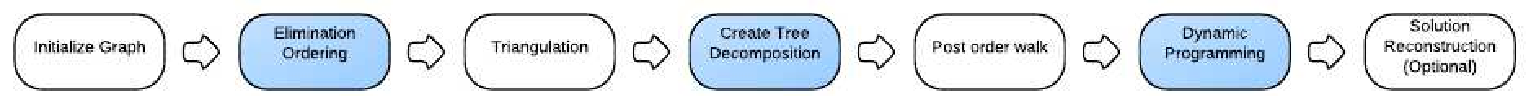
\includegraphics[scale=0.60]{figures/SequentialAlgorithmDiagram.pdf}
\caption{Solving MWIS using Dynamic Programming and Tree Decompositions}
\label{fig:sequential.algorithm}
\end{figure*}

After construction, the resulting decomposition $(X,T)$ is rooted, and we execute the dynamic programming
following a post-order walk on the tree $T$. At each node, we construct a hash table of partial
solutions --- for MWIS, this stores each independent set within the bag with the weight
of the best possible ``expansion'' of that set into the subtree rooted
at that bag. As shown in Algorithm~\ref{alg:compute_dp_table}, we can reduce memory requirements
by storing only the independent sets in the intersection of a bag with that of its parent node. %(also described in ~\cite{serialTM}).
When the post-order walk terminates at the root, the highest weight in the root node's hash table is the
maximum weight of any independent set in the graph $G$. If the elements in the maximum
weighted independent set are desired, extra bookkeeping is required during the computation,
and the algorithm must walk back ``down'' the tree to construct the solution from the hash tables.

\begin{algorithm}[!ht]
\caption{Compute a node's hash table}\label{alg:compute_dp_table}
\begin{algorithmic}[1]
\Procedure{ComputeDPTable}{$G$, $T$,$k$}\\
\text{$\triangleright$ Graph $G$, a tree decomposition $T$, node $k$}
\State Let $T=(X,(I,F))$ where $c_1, c_2, \ldots, c_d$ denote
\State the children of node $k$ and $p$ the parent
\State Let $D_j$ be the DP hash table for node $j$
\State with $f_j(s)$ the value of a set $s$ in $D_j$
\State $S=\textsc{FindAllWIS}(G[X_k])$ \\
\hskip1em \text{$\triangleright$ $S$ a set of ordered
  pairs $(s,w(s))$}\label{algline:findallWIS}
\ForAll{$(s,z)\in S$}
  \For{$i=1$ to $d$}
    \State{$t_i=s\cap X_{c_i}$}%\text{\%$t_i$ is the part of $s$
%      contained in child $i$'s bag}
    \State Look up $t_i$ in table $D_{c_i}$: $(t_i,\cdot,f_{c_i}(t_i))$
    % CSG not sure about this notation...
    \State $z=z+f_{c_i}(t_i)$
  \EndFor
  \State\text{$\triangleright$ Subtract the weight of the parent
    intersection}
  \State Let $s_p=s\cap X_p$; $f_k(s_p)=z-w(s_p)$
  \label{algline:computeparentintersection}\label{algline:computeDPvalue}
  \If{$(s_p,\cdot,\cdot)\notin D_k$}%\State\text{\%Add hash table entry}
        \State $D_k=D_k\cup (s_p,s,f_k(s_p))$\label{algline:addhashentry}
  \Else\hfill \text{$\triangleright$ The key $s_p$ exists in the hash table}
    \State Let $(s_p,s',x)$ be current entry in $D_k$
    \If{$f_k(s_p)>x$}
      \State{Update $D_k$ to ($s_p,s,f_k(s_p)$)}\label{algline:updatehashentry}
    \EndIf
  \EndIf\label{algline:checktableend}
\EndFor
\State{\textbf{return} $D_k$}
\EndProcedure
\end{algorithmic}
\end{algorithm}

\subsection{Sequential Implementation Results}\label{sec:seq_results}

In previous work~\cite{serialTM}, we presented sequential software to
construct tree decompositions using various heuristics alongside a fast,
memory-efficient dynamic programming implementation for solving MWIS.
Although that work showed that algorithms based on these techniques could be practical from a computational standpoint,
it also revealed numerous bottlenecks in the computation that limited the scale of the graphs which could be analyzed.
Two limiting factors are the amount of memory required to store the dynamic programming tables of partial results from
numerous subproblems at multiple tree nodes simultaneously, and the total time required for the generation and subsequent node-by-node analysis of
the tree decomposition. We now quickly review the serial performance on
a test suite of partial $k$-trees of various widths and
sizes. We consider two metrics: runtime measured in seconds
and memory high water mark (HWM) measured in gigabytes (GB), which is the
maximum memory in use at any given time during execution. In Figures~\ref{fig:pkt.width} and
~\ref{fig:pkt.nodes}, we provide separate timing and HWMs for the tree decomposition (TD)
and dynamic programming (DP) steps as the width and size of the graph change. For example,
Figure~\ref{fig:pkt.width} illustrates the increase in runtimes and memory usage when the
graph size is fixed and its width increases.
We note that for higher width graphs, dynamic programming takes up to twice as much time
as tree decomposition, and uses nearly four times the memory.

\begin{figure}[!ht]
\subfigure[Time]{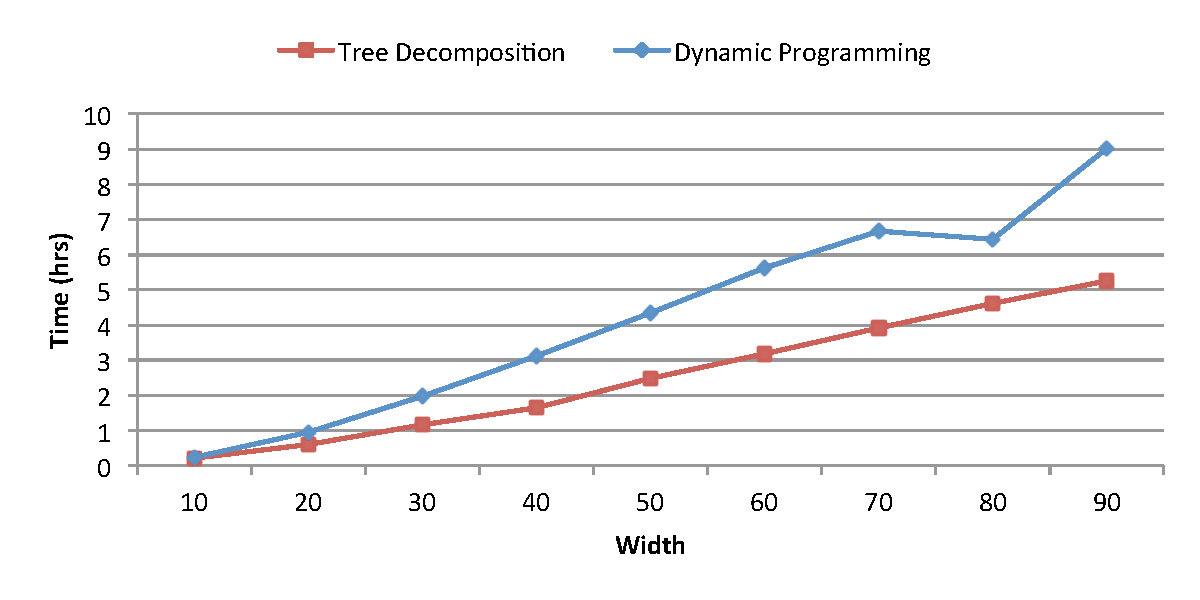
\includegraphics[angle=0,width=3.1in]{figures/fig1_time_col.pdf}\label{fig:pkt.width.time}}
\subfigure[Memory]{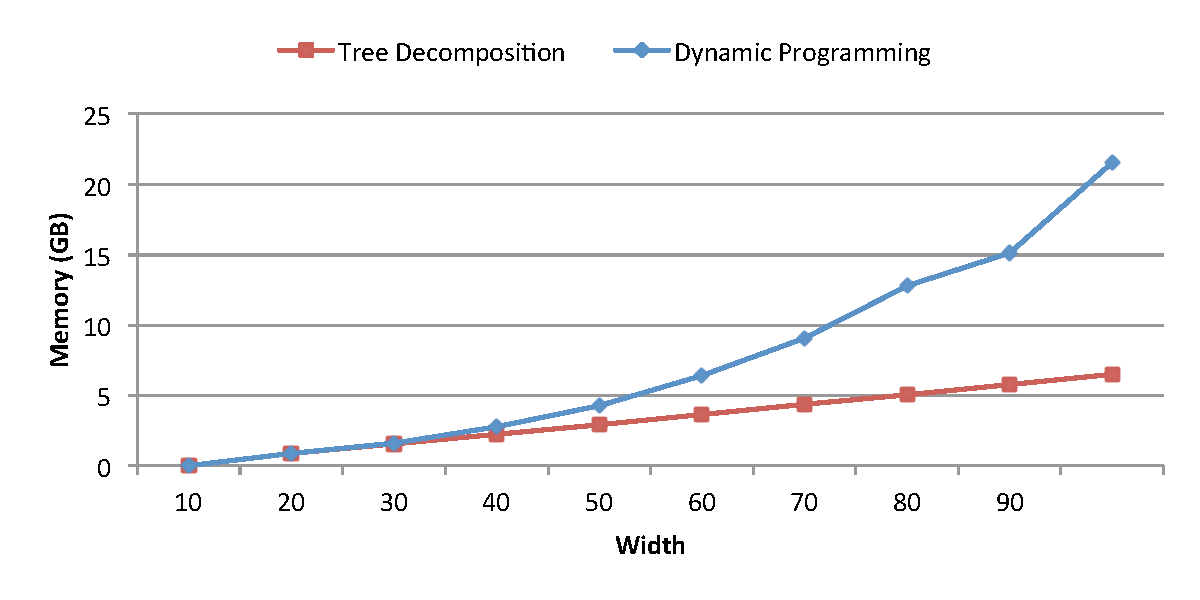
\includegraphics[angle=0,width=3.1in]{figures/fig1_mem_col.pdf}\label{fig:pkt.width.mem}}
\caption{Runtime and memory variation with the width of graph
  $pkt.500000.width.80$}
\label{fig:pkt.width}
\end{figure}
%DPW on this figure and the next, TD time's color is a bit too light in black and white.

Since the real benefit of tree decomposition-based algorithms lies in fast solutions
for low-width graphs with a high vertex/edge count, we also include a plot of performance at a fixed width,
with increasing graph size, in Figure~\ref{fig:pkt.nodes}. It is interesting to
note that this changes the balance of resources needed for each step of the algorithm drastically.
Here, decomposition generation dominates the runtime, and the memory used during dynamic programming
is only negligibly higher than that needed for tree construction (hard to see even at a logarithmic scale, as used in Figure ~\ref{fig:pkt.nodes.mem}).

\begin{figure}[!ht]
\subfigure[Time]{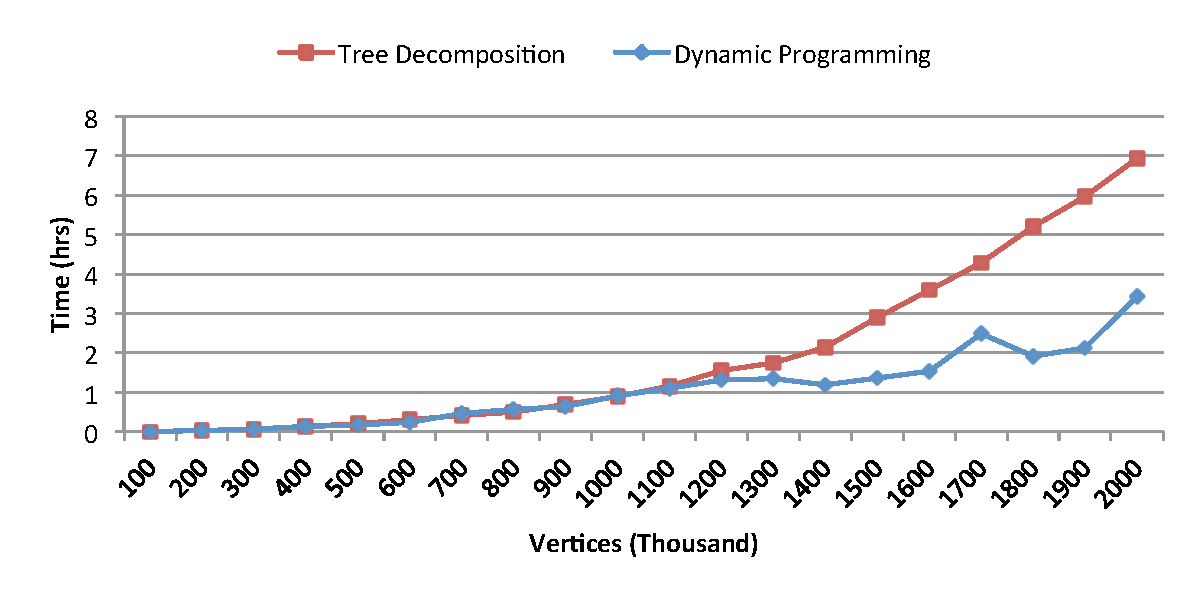
\includegraphics[angle=0,width=3.1in]{figures/newfig3a_col.pdf}\label{fig:pkt.nodes.time}}
\subfigure[Memory]{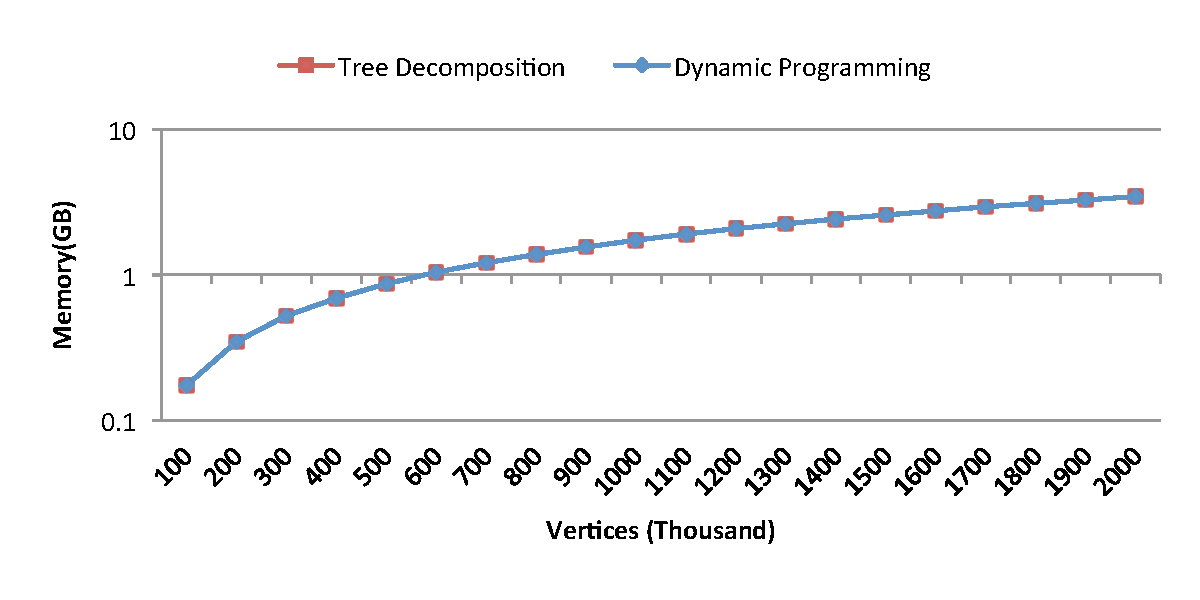
\includegraphics[angle=0,width=3.1in]{figures/newfig3b_col.pdf}\label{fig:pkt.nodes.mem}}
\caption{Runtime and memory variation with the number of nodes of the graph $pkt.nodes.10.80$}
\label{fig:pkt.nodes}
\end{figure}

These results indicate that both the tree decomposition generation and the dynamic programming
would benefit from a parallel implementation --- the former primarily to reduce the runtime, and the latter
to provide both acceleration and the distribution of objects across the memory of numerous nodes.

\section{Creating tree decompositions in parallel}
As discussed in Section~\ref{sec:seq_results}, generating the tree decomposition can
become a bottleneck as the number of nodes in the graph grows. In order to address this,
we developed parallel algorithms for two key steps in the process: (i) finding an elimination ordering,
and (ii) generating the bags for the tree decompositions. Finding the bags is computationally intensive
since it repeatedly searches for the neighbors of a vertex $v$ which occur after $v$ in the ordering,
i.e., the {\it forward neighbors}. Here we describe our approaches to improving the performance of both on a distributed memory architecture.

\subsection{Parallel elimination order generation}\label{sec:elimination_order}

A close look at the profile of the subroutines needed for tree decomposition, shown at log scale in Figure \ref{fig:pkt.td}, shows elimination ordering (using the METIS implementation of the multiple minimum degree heuristic) takes roughly 90\% of
total time. To address this, we integrated routines from the
ParMETIS library~\cite{Karypis1996parallel}~\cite{Karypis1997parmetis},%~\cite{Karypis1996parallel_k}
 which provides a distributed fill-reducing ordering using nested dissection techniques. Although this provided
a drastic reduction in runtime, the widths of the resulting tree decompositions (shown in Figure~\ref{fig:eo_width})
were often unacceptably larger than their sequential analogues. We note that more generally, the heuristics
employed to find the ordering were originally designed to minimize the number of edges added
in the triangulation and offer mixed results with respect to width (see \cite{serialTM}).

%NEW TEXT
Since the complexity of the dynamic programming
is exponential in the treewidth, it is critical to devise a parallel ordering routine that limits this
inflation. Based on ideas in a paper of Hendrickson et al.~\cite{HendricksonEO},
we created a two-step procedure that first uses ParMETIS to partition the nodes into subsets which have known
relative positions in the final order, then runs a second fill-reducing heuristic (we chose the AMD algorithm~\cite{Amestoy2004algorithm}) on the subgraph induced by each subset  to refine the ordering. Note that the second step's runs may be done in parallel as the subsets are disjoint. For computational results and conclusions, please see Section~\ref{sec:exp_elimination_order}.

\begin{figure}[ht]
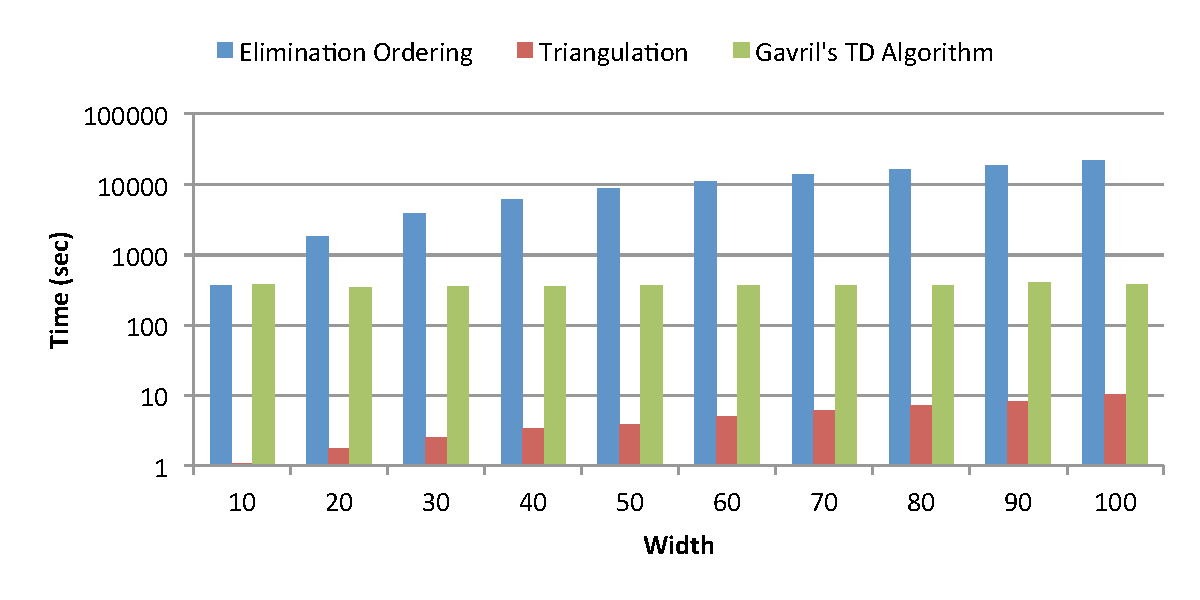
\includegraphics[angle=0,width=3.1in]{figures/fig3_col.pdf}
\caption{Breakdown of TD construction time on $pkt.500000.width.80$ graphs}
\label{fig:pkt.td}
\end{figure}

\subsection{A parallel version of Gavril's algorithm}
Once the elimination ordering time has been reduced, Gavril's algorithm ~\cite{Gavril1974} %(Algorithm~\ref{alg:gavril})
dominates the tree decomposition computation. We parallelize this algorithm
using a hybrid MPI + \emph{pthreads} approach, with each thread executing the function in Algorithm~\ref{alg:pbag_gen}.
%BDS
Vertices of the original graph are distributed evenly between MPI processes, then further divided based on 
available pthreads on the system (this sets the prefix, start, and end values).
This distributes the work of finding forward neighbors and calculating tree edges across multiple compute nodes, with multiple bags being generated simultaneously on each node.
In Gavril's original algorithm, when the bag for a vertex is created, it is compared with bags already in the decomposition to see
if it can be created by just adding the vertex currently under consideration. Since these bags may not be locally known
%Since the bag $X_{t[m]}$ in line ~\ref{gav:line:bag_merge} of Algorithm~\ref{alg:gavril}
is not locally known in a distributed environment, we postpone the bag unions to
a sequential refinement stage, temporarily creating a tree with exactly $n$ nodes. The master process then operates on the full set of
$n$ bags and $n-1$ edges, merging appropriate nodes to produce a tree equivalent to the sequential
algorithm (for the same elimination ordering). In Algorithm~\ref{alg:par_td},
the subroutine \textsc{ReplaceParent} is used to remove redundancy when a parent and child in the unrefined tree have identical bags by essentially removing the child from the tree, making its children now directly inherit from what was their grandparent. Computational results of this parallelization can be found in Section ~\ref{sec:exp_td}

%%%%%%%%%%%%%% Threaded Bag Processing  %%%%%%%%%%%%%%%%%%%
\begin{algorithm}[ht!]
\caption{Threaded bag processing}
\label{alg:pbag_gen}
\begin{algorithmic}[1]
\Procedure{ThreadBag}{G, $\Pi$, prefix, start, end} %,rank, id}%vestige of implementation
\For{$i$ = $start$ to $end$}
\State $B_i$=$\text{\textsc{GetNeighbors}}(G,\pi_i,\{\pi_{i+1},${\tiny \ldots},$\pi_n\})$
\State Find $m = \pi_{j}$ such that $j \leq k$ for all $\pi_{k} \in
B_{i}$
\State $X_{k} = B_{i} \cup \{\pi_{i}\}$
\State \textsc{store} $(\pi_{i}$,$\pi_{m})$
\Comment edge to parent bag
\State \textsc{store} $X_{k}$
\Comment content of the current bag
\EndFor
\State \textsc{send} all stored edges and bags to rank 0.
\EndProcedure
\end{algorithmic}
\end{algorithm}
%%%%%%%%%%%%%% End Threaded Bag Processing %%%%%%%%%%%%%%%%%%%

%%%%%%%%%%%%%% Parallel Tree decomposition %%%%%%%%%%%%%%%%%%%%%%
\begin{algorithm}[ht!]
\caption{Parallel tree decomposition}
\label{alg:par_td}
\begin{algorithmic}[1]
\Procedure{ParallelTreeDecomposition}{}
\State Let $\Pi$=$(\pi_1, \pi_2, \ldots, \pi_n)$; $wr, ws$ be MPI rank and communicator size with $nthreads$ pthreads per task.
\State $xr = n/ws$, $startpos = wr*xr$
\State $tr = xr/nthreads$
\For{$i$ = 0 to $nthreads$}
\State $tstart = startpos + i*tr$
\State $tend = tstart + i*tr$
\State \textsc{ThreadBag} $(G, \Pi, prefix, tstart, tend)$
%\State $\textbf{Thread\_create}(G, \Pi, prefix, tstart, tend,$
%\State $wr, i, ThreadProcessBag)$
\EndFor
%\For{$i$ = 0 to $nthreads$}
%\State $\textbf{Thread\_finish}()$
%\EndFor
\State $\textbf{Barrier()}$
\State {{\textsc Gather} tree edges and bags from threads
to create a tree decomposition $(T,X)$ with $n$ nodes, $n-1$ edges.}\label{pbag_gen:line:gather}
%% Merge files
\If {$wr == 0$ (serial refinement)}
%% Refinement
\State Let $X_i$ be the bag of node $i$, associated with vertex $\pi_i$.
Let $Adj_i$ be the neighbors of $i$ in $T$, with $P_i$ the parent node.
Let $R$ be root of $T$.
\For{$i$ = $n-1$ to $1$}
%\State $X^{\prime}_i$ = $X_i  \backslash \pi_i$
\If{$X_i \backslash \pi_i == X_{P_i}$} %changed this to not define X' to avoid confusion in return statement.
\State \textsc{ReplaceParent}(i)
%Specifics of replacing the parent with the current node.
%\State $Adj_i = Adj_i \backslash \pi_{P_i}$
%\For{$\pi_k$ in $Adj_{P_i}$ with $\pi_k \neq \pi_i$}
%\If{$Adj_k \neq \emptyset$}
%\State $Adj_i$ = $Adj_i \cup \pi_k$
%\State $Adj_k$ = $(Adj_k \backslash \pi_{P_i}) \cup \pi_i$
%\If{parent of $\pi_k == \pi_{P_i}$}
%\State $\pi_k$ set parent to $\pi_i$
%\EndIf
%\EndIf
%\If{$\pi_{P_i} == R$}
%\State $R = \pi_i$
%\Else
%\State $\pi_i$ set parent to $P_{P_i}$
%\EndIf
%\State $Adj_{P_i} = \emptyset$, $X_{P_i} = \emptyset$
%\EndFor
\EndIf
\EndFor
\EndIf
\State Write $(T^{\prime}, X^{\prime})$ with
$X^{\prime} = \{X^{\prime}_1, X^{\prime}_2, \ldots, X^{\prime}_m\}$
where $X^{\prime}_i \in X$ and $Adj^{\prime}_{i} \neq \emptyset$
\EndProcedure
\end{algorithmic}
\end{algorithm}
%%%%%%%%%%%%%% End Parallel Tree decomposition %%%%%%%%%%%%%%%%%%%%%%


\section{Task-oriented parallel dynamic programming}

Having described our approach
% CSGCSG - was novel ideas 
for parallel construction of tree decompositions, we now move on to our approach to dynamic programming in a distributed memory environment. We use task-oriented computing, where large operations are divided into smaller units called tasks. These tasks are then executed asynchronously across a distributed computer. 
%MADNESS is a fast and accurate environment for computational chemistry, now used in many other
%fields including nuclear, atomic, and molecular
%physics. %[references] fill in if time
The MADNESS library and parallel runtime provide a versatile scientific computing environment that abstracts the intricacies of task-oriented computing, allowing application developers to focus on algorithm development and implementation.
The commonly used tools (for computational chemistry and physics) in MADNESS are implemented on top of its parallel runtime, which provides an API for parallel data structures and functionality required for task-oriented computation. Key features include a) futures to manage dependencies and hide
latency; b) global name spaces; c) non-process-centric
computing; and d) dynamic load balancing and data redistribution~\cite{Thorntonintroducing}.
We use MADNESS tasks to encapsulate the computation required at each
tree node, and define dependencies using futures.

%\subsection{Task oriented computing and MADNESS parallel runtime}

% \subsection{Parallel dynamic programming algorithm}

Important steps in any parallel algorithm for solving the maximum weighted independent set problem
using dynamic programming are a) creating a table for storing all independent sets; and
b) updating weights of the independent sets at a tree node based on the values from children.

% Begin Edit Dinesh
% Explain how we use OpenMP with Madness
% CSGCSG rewording lots here
One can configure the MADNESS runtime to match processor layout in a compute node
in order to assign MADNESS tasks as desired.
The MADNESS runtime also provides the ability to assign threads to each MADNESS tasks. 
However, the user does not have any control over the work done by the threads 
since they are controlled by the runtime.
In order to limit the amount of communication amongst MADNESS tasks and to make tree nodes
self-contained, we define a local data structure in every bag that takes advantage of the
runtime's distributed container.
The local data structures are small (e.g. a $w\times w$ binary matrix, where $w$ is the bag size) 
and are identical to those used in the serial implementation. The local data structures
include the bag intersections with children/parent nodes, a list of adjacent tree nodes, and the associated induced subgraph as a binary matrix.  
Since the work for ``preparing'' each node is independent, we employ OpenMP within the task to speed up this pre-processing phase. All tasks can then access information using a key in the distributed container regardless of the physical location of the data. Tree nodes are distributed across tasks using a mapping function provided by the MADNESS parallel runtime. The task owning each node is responsible for populating the local data structures and adding it to a MADNESS distributed container (a built-in distributed hash-map-like data structure).

%Tree nodes are distributed across tasks using a mapping function
%provided by the MADNESS parallel runtime. The task owning each node is responsible
%for populating the local data structures and adding it to a MADNESS distributed container
%(a built-in distributed hash-map-like data structure). The local data structures are small (e.g. a $w\times w$ bitwise matrix, where $w$ is the bag size), and identical to those populated in the serial implementation; they include the bag intersections with children/parent nodes, list of adjacent tree nodes, and the associated induced subgraph.  Since the work for ``preparing'' each node is independent, we employ OpenMP within the task to speed up this pre-processing phase. All tasks can then access information using a key in the distributed container
%regardless of the physical location of the data.
% End Edit Dinesh

Once all nodes are prepared, and the distributed container is populated, we
define MADNESS tasks recursively via a pre-order walk starting at the root,
using Algorithm~\ref{alg:ComputeTable}.
At the leaf nodes, full hash tables with all independent sets are computed and returned
to the parent node via a \textsc{LeafTable} routine. After launching tasks for their children,
internal nodes of the tree wait for each child to finish, then incorporate the partial solutions
into the current table in \textsc{UpdateTable}. %NEW TEXT
The MADNESS task model enables us to
implement asynchronous table updates --- the parent can update the table with
input from each child as it finishes, in an arbitrary order. Some care
must be taken to avoid race conditions, but the overall impact is
a faster implementation (since the work at a parent can be partially
completed prior to receiving updates from its last child). It should be noted that
although the tree nodes will likely be processed on different compute nodes,
the MADNESS runtime frees the application developer from having to
worry about the physical location of each table.

\begin{algorithm}[ht!]
\caption{Compute hash table for bag $X_{i}$}\label{alg:ComputeTable}
\begin{algorithmic}[1]
\Procedure{ComputeTable}{$i$}
\State Let node $i$ have bag $X_i$ and neighbors $Adj_i$
\If{$i$ is a leaf}
\State \textbf{return} \textbf{MADTask}(\textsc{LeafTable}($i$))
\EndIf
\State Let $U[], V[]$ be arrays and $j = 0$
\For{$n$ in $Adj_{i}$}
\State $U[j]$ = \textbf{MADTask}(\textsc{ComputeTable}($n$))
\State $V[j]$ = \textbf{MADTask}(\textsc{UpdateTable}($i$, $U[j]$))
\State $j = j + 1$
\EndFor
\State Wait for all \textbf{Futures} in $V$ to return
\State \textbf{return} $X_{i}$
\EndProcedure
\end{algorithmic}
\end{algorithm}

\section{Experimental Results}~\label{sec:experiments}

In the final section of the paper, we describe some
computational results that demonstrate the scaling behavior
of the parallel procedures described in the previous sections.
We partition our scaling results into two parts, first reporting on the performance of the parallel tree
construction, then on the dynamic programming.  While we do achieve reasonable speedups
for the tree construction phase, we believe the scaling of the dynamic programming will
dominate the overall behavior when using these algorithms to solve large realistic problem instances.
As the graph size grows in terms of number of nodes and edges, one can reasonably
expect the treewidth of the graph to also increase.  While the tree decomposition
construction times grow relatively slowly with both the graph size and its width
(see Figures 2 and 3, for example), the dynamic programming running time and
memory consumption increase exponentially with the width, making it a more
significant computational hurdle.  Furthermore, the dynamic programming step
is more difficult to parallelize due to the asynchronous nature of the computation.
While it is often difficult to achieve good scaling results for graph optimization problems
and dynamic programming in general, we demonstrate linear (and in some cases even superlinear)
speedups for the dynamic programming phase of our optimization algorithm.
% CSGCSG rewording
We consider our parallelization of the dynamic programming to be the major
computational contribution of our work.

The sequential results used for comparison here were obtained using one core of a
2.80Ghz Intel Xeon X5560 %quad-core processors (a total of 16 cores, though only one was used by the serial code),
processor with 8MB of L1 cache and 24GB of memory. Sequential runtimes were limited to a maximum of
24 hours. The parallel experiments were run on a 1024 node partition of Jaguar~\cite{jaguar}, a Cray XK6 with one 16-core AMD 6200 series processor and 32GB of memory per node.


\subsection{Parallel elimination order generation}\label{sec:exp_elimination_order}
To evaluate our algorithms for generating elimination orderings in parallel,
we compare both the widths of the resulting decompositions and the required runtime.
In Figure~\ref{fig:eo_width} we illustrate the differences between $k$ (an upper bound on the treewidth,
since the graphs are partial $k$-trees), and the widths produced by ParMETIS\_V3\_NodeND (v3) and our hybrid combining ParMETIS with AMD (v3+amd). The partial $k$-trees were
generated with parameters chosen to maintain a constant edge density
(e.g. 500K nodes, $k = 10$ has the same edge density as 1.2M nodes, $k = 24$).
Using AMD improves the width over ParMETIS alone for graphs with smaller $k$ values, but
as the width increases, the advantage is lost.
In Figure~\ref{fig:test_eo_width} we look at a second test suite of
partial $k$ trees, where we compare both runtimes and width against the sequential heuristic MetMMD.

\begin{figure}[!ht]
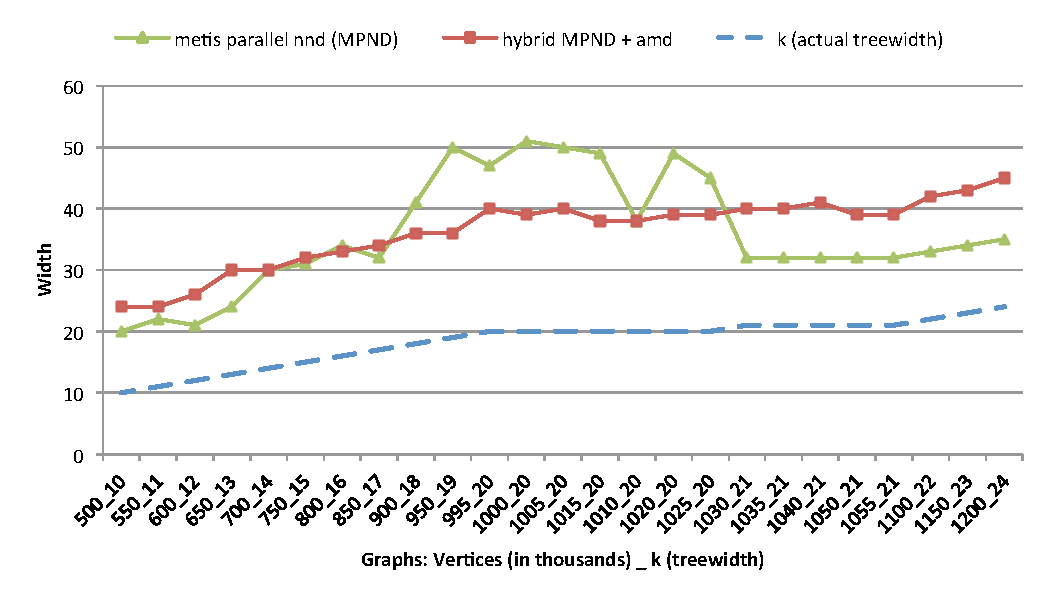
\includegraphics[angle=0,width=3.1in]{figures/newfig6_col.pdf}
%\includegraphics[scale=0.40]{figures/widths_v3_v3_amd.eps}
\caption{Widths achieved on $k$-trees using ParMETIS and ParMETIS + AMD}
\label{fig:eo_width}
\end{figure}

\begin{figure}[!ht]
\subfigure[Time]{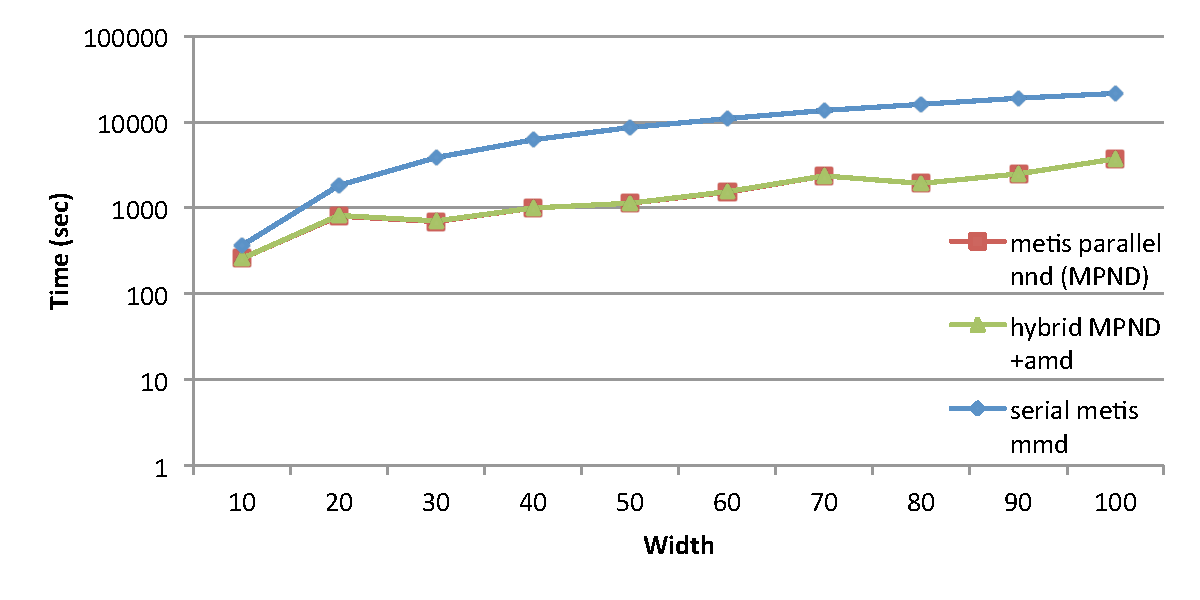
\includegraphics[angle=0,width=3.1in]{figures/fig4_time_col.pdf}}
\subfigure[Width]{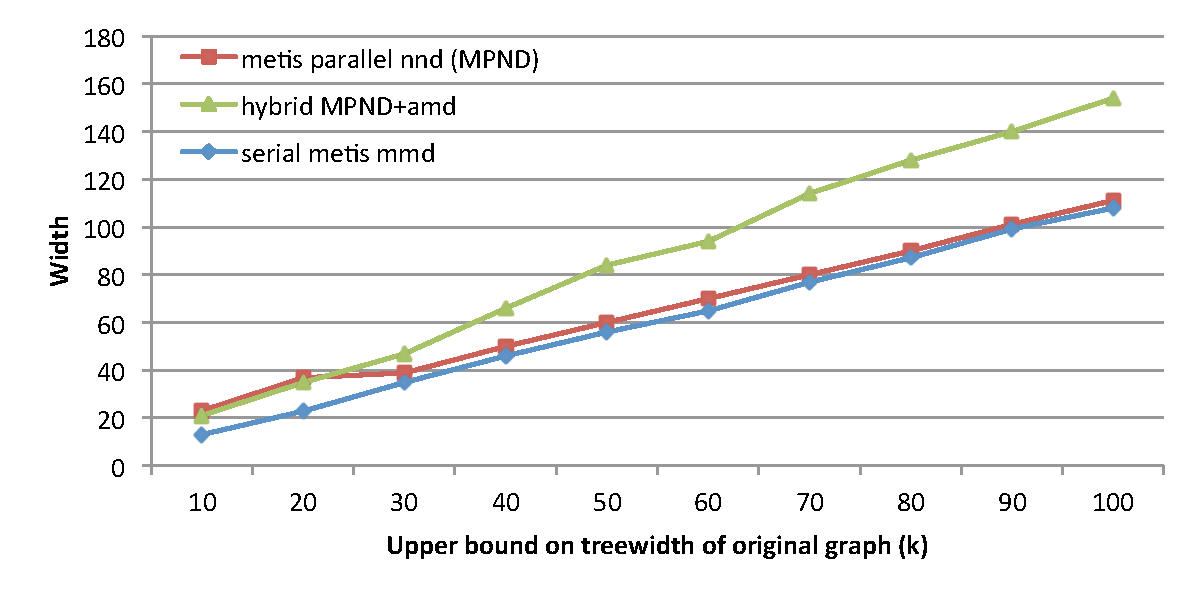
\includegraphics[angle=0,width=3.1in]{figures/fig7_col.pdf}}
\caption{Timing for parallel and sequential elimination ordering heuristics on graphs $pkt.500k.width.80$}
\label{fig:test_eo_width}
\end{figure}


\subsection{Parallel tree decomposition and dynamic programming}\label{sec:exp_td_dp}

H\"uffner, et al., opined that
``As a rule of thumb, the typical border
of practical feasibility lies somewhere below a treewidth of 20 for the underlying
graph" \cite{huffner}. Prior work using tree
decompositions to solve optimization problems was typically limited to graphs less than 5000 nodes,
with the techniques described in a recent paper ~\cite{cliquecover} restricting experiments even further --- to just several hundred nodes. We report computational results on partial $k$-trees with five hundred thousand, one
million, and two million nodes with $k = 10,25$, and $50$. These represent graphs we believe are of an unprecedented scale - one which was previously deemed impractical.

\subsubsection{Parallel tree decomposition}\label{sec:exp_td}

\begin{figure}[!ht]
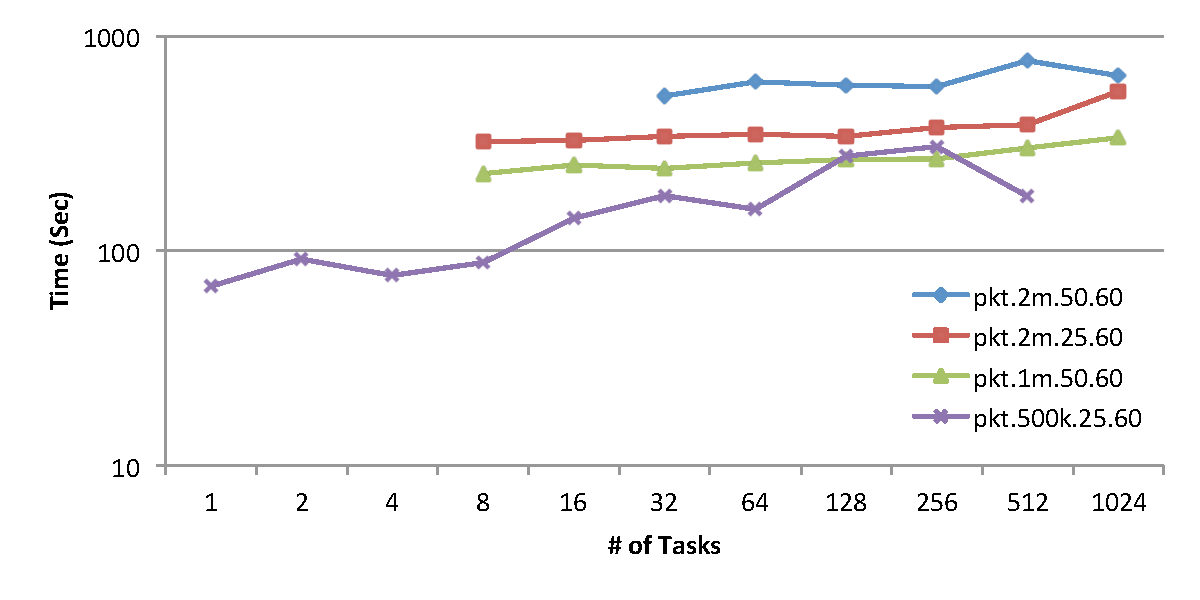
\includegraphics[angle=0,width=3.1in]{figures/newfig8_col.pdf}
\caption{Parallel tree decomposition runtimes }
\label{fig:TDtimes}
\end{figure}

The INDDGO package implements all the necessary algorithms to
% CSGCSG - we are missing some algs now
% Algorithms~\ref{}alg:eo_parmetis} through ~\ref{alg:par_td} to 
enable the generation of tree decompositions where all steps leverage available parallel resources. Figure~\ref{fig:test_eo_width} shows the time required and widths achieved by parallel elimination orderings relative to a serial heuristic.

In Algorithm~\ref{alg:par_td}, our current implementation collects all of the
edges and bags created by each compute node (line~\ref{pbag_gen:line:gather})
by writing one file per MPI task.  The rank-zero task then performs a concatenation
prior to refinement. Unfortunately, this usage of the file system appears to prevent the scaling of our
parallel tree decomposition construction beyond a modest number of MPI processes, as seen in Figure~\ref{fig:TDtimes}.
We believe that replacing the file system interactions by a set of local memory stores followed by a global gather would resolve this problem, and is planned as a future improvement to the code.

Despite the delays inherent from file system use, we achieve up to a $70\times$
speedup over the sequential version on just 32 cores (see Table~\ref{tbl:td_scale}).
This superlinear speedup can be attributed to a new, more efficient version of the \textsc{FindNeighbors} routine
that takes advantage of caching within each task.

\begin{table}
\centering
\begin{tabular}{|c|c|}
\hline
Graph & Speedup \\
\hline
pkt.500000.25.60 & 3.02\\
pkt.1000000.50.60 & 10.73\\
pkt.2000000.25.60 & 70.46\\
pkt.2000000.50.60 & 44.00\\
\hline
\end{tabular}
\caption{Speedup with 8 tasks x 4 threads for Algorithm~\ref{alg:par_td}}
\label{tbl:td_scale}
\end{table}

\subsubsection{Parallel dynamic programming}\label{sec:exp_dp}

\begin{figure*}[!t]
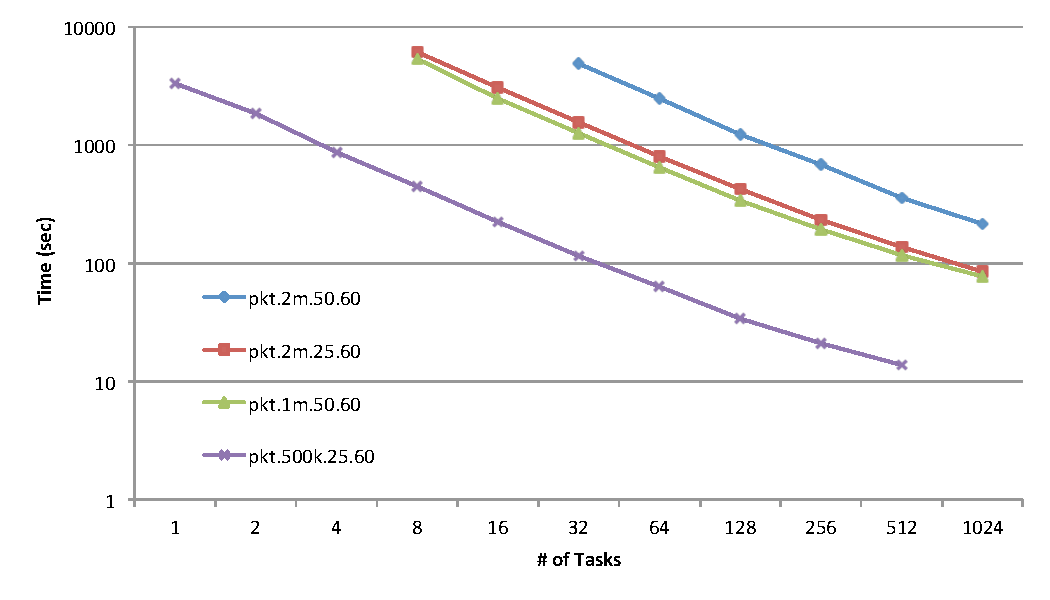
\includegraphics[angle=0,width=6in]{figures/newfig9_col.pdf}
\caption{Dynamic programming runtime}
\label{fig:DPtimes}
\end{figure*}

Although the parallelization of the tree decomposition
construction may not show compelling scaling results, our dynamic
programming implementation shows exceptional scaling.
For example on a partial 25-tree with 500,000 nodes, the dynamic programming portion of the
sequential algorithm required almost 22 hours (76630 seconds), and the
speedup shown in Figure~\ref{fig:500k.25.seq.sp} is superlinear. For example 512 tasks with
8 threads each completed the dynamic programming in only 13 seconds!

We first consider the behavior of our algorithms with respect to the shared memory parallelism.
Figure~\ref{fig:thread_scale} shows the runtime of the dynamic programming algorithm using
a fixed number of MADNESS tasks (128) and varying the number of OpenMP threads per task.
Threading improves the runtime until we reach 12 threads, where delays from increased memory contention
offset the gains from parallel processing.  Based on Figure~\ref{fig:thread_scale}, we chose to conduct
the remainder of our scaling experiments using 8 OpenMP threads per MADNESS task to optimize performance.

\begin{figure*}[!ht]
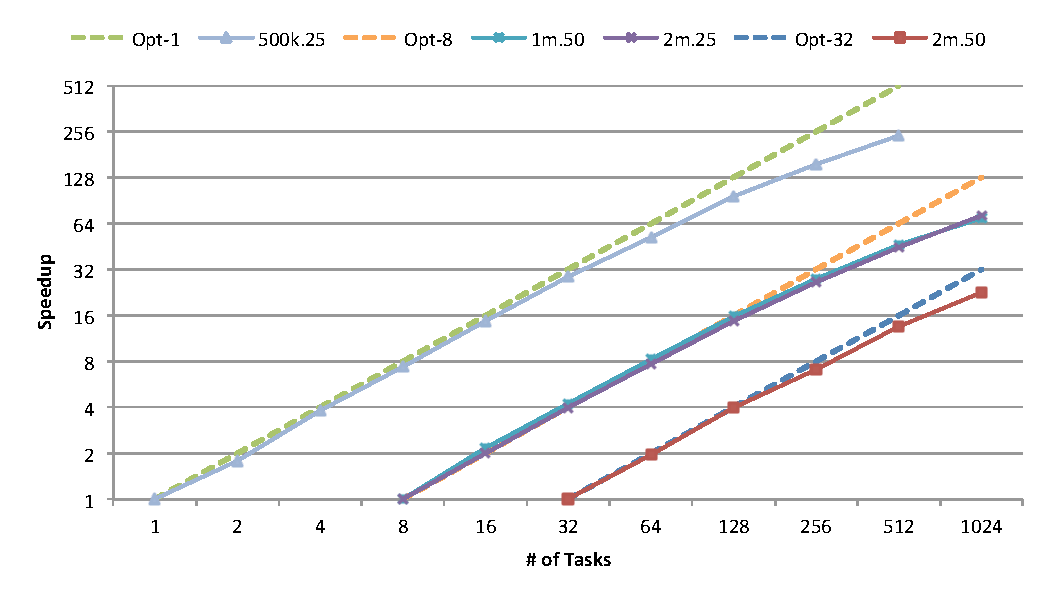
\includegraphics[angle=0,width=6in]{figures/fig10_col.pdf}
\caption{DP speedup, shown relative to smallest successful parallel execution time}
\label{fig:DPspeedup}
\end{figure*}

Figures~\ref{fig:DPtimes} and~\ref{fig:DPspeedup} illustrate the runtime and speedup, respectively, as we vary both the number of tasks and the size of the input problem. We note that all sequential experiments were run with a
with a time limit of 24 hours, which prevented almost all graphs with width greater than 10 from completing. In Figure~\ref{fig:DPtimes}, this leads to trend lines that do not extend to the smaller numbers of tasks for graphs on a
million or more nodes.  To present speedup results, we used the smallest (and thus slowest) parallel run completed in less than 24 hours (the minimum number of tasks depended on the input size) as a baseline for computing our speedups. Figure~\ref{fig:DPspeedup} depicts scaling relative to the appropriate base case by using dashed lines to indicate linear speedup (e.g. Opt-1 is linear relative to performance with 1 task and Opt-32 relative to an initial run with 32 tasks) on the same graphs used in Figure~\ref{fig:DPtimes}. As one can see, when the graph is large enough, the MADNESS tasks were not starved for work and we were able to achieve speedups that are approximately linear.  Increases in communication overhead as the number of tasks increases prevent perfect scaling.

\begin{figure}[!ht]
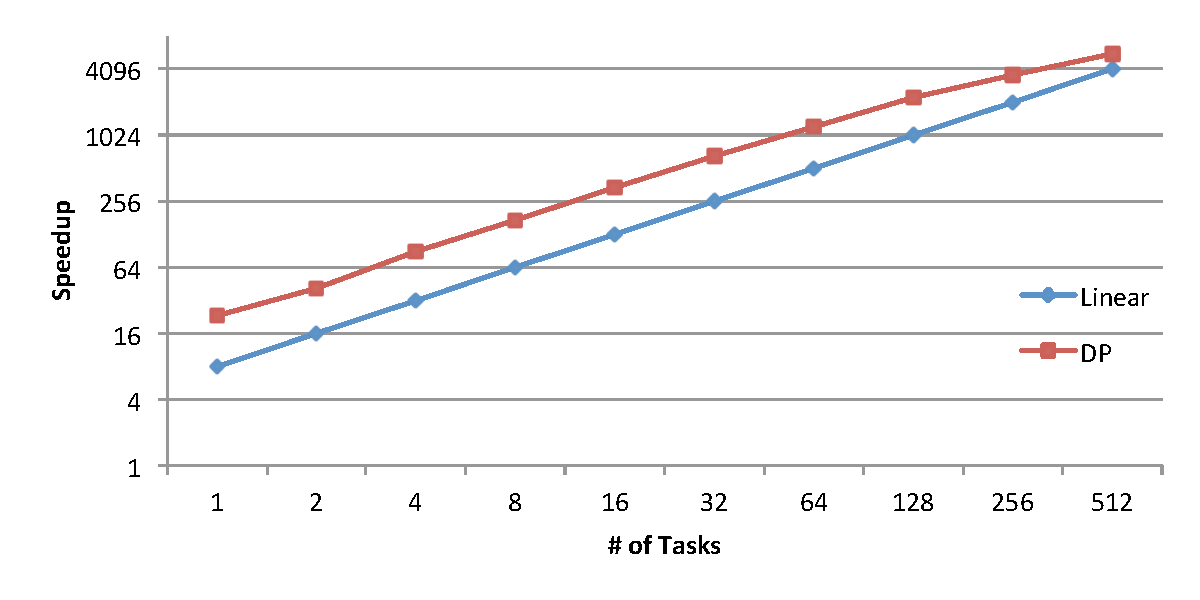
\includegraphics[angle=0,width=3.1in]{figures/fig11_col.pdf}
\caption{DP speedup for pkt.500000.25.60}
\label{fig:500k.25.seq.sp}
\end{figure}

\begin{figure}[!ht]
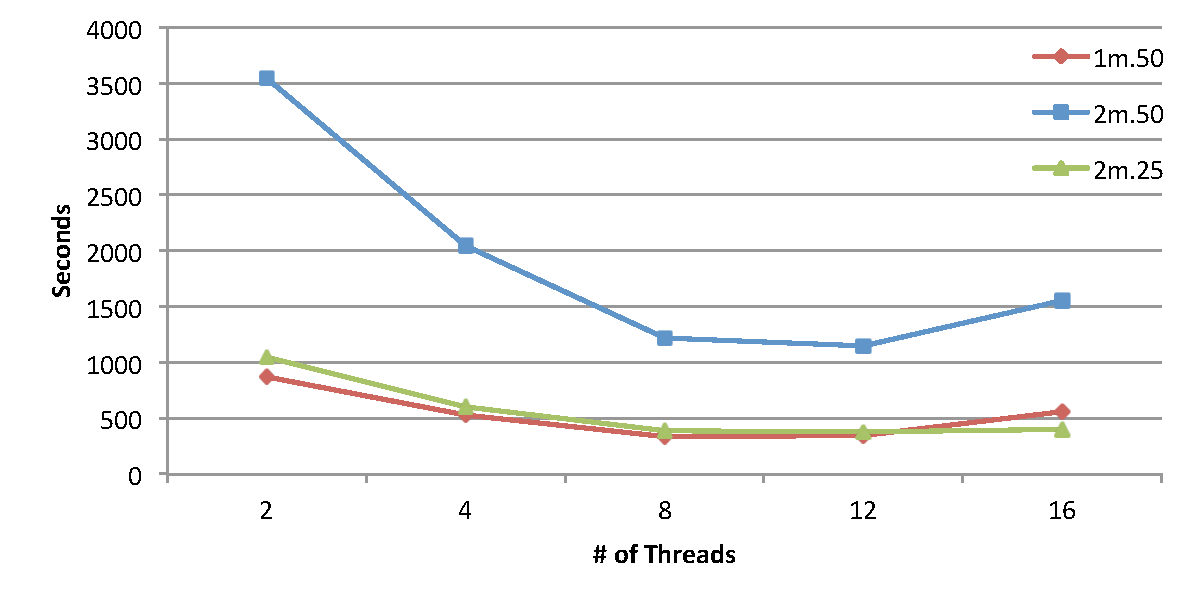
\includegraphics[angle=0,width=3.1in]{figures/fig12_col.pdf}
\caption{DP runtime with 128 tasks and varied OpenMP thread count}
\label{fig:thread_scale}
\end{figure}

\section{Conclusions and Future Work}
In this paper we present what we believe to be the first application of high performance
 parallel computing to tree decompositions and the related dynamic programming.
We propose novel parallel
algorithms to find elimination orderings, generate tree decompositions from these orderings, and to perform
the memory-intensive dynamic programming using the MADNESS
runtime. Our techniques are able to exactly solve MWIS instances that are
orders of magnitude larger (in terms of number of vertices and edges) than any other problems solved 
to optimality in the
literature.  
% CSGCSG - probably true, but...
%Since the scaling of other branch-and-bound based
%algorithms depends strongly on the number of nodes and edges in the
%graph, we believe our work presents the only known method to solve problems of
%this size to optimality.


Our empirical study shows the performance of each algorithm when run on graphs
with various widths and sizes, and many cases exhibit excellent scaling.
Our latest code is available for other researchers as part of the INDDGO software package~\cite{inddgo},
and one of our longer term
goals is to develop a more general framework for solving graph optimization
problems via the type of dynamic programming we discuss in this paper.
Such a framework would allow the application developer to
write only the problem-specific code for the dynamic programming; everything related
to the tree decomposition and the distribution of tasks would be handled by
the framework.
%and dynamic programming will operate under the hood.

%In this paper we investigate the use of AMD algorithm to enhance the
%results of ParMETIS, though one could certainly choose another serial
%heuristic to replace it.
%We use elimination ordering to implement parallel tree decomposition generation however
%an investigation on alternate tree decomposition methods will be
%worthy. effort. A promising alternate method propose
%in~\cite{Dourisboure2007tree}.
%
%Also, in future we hope to develop a
%more general framework for problem solving using tree
%decomposition. Such a framework will allow application developer to
%write only problem dependent code and everything related to tree
%decomposition and dynamic programming will operate under the hood.

\section{Acknowledgements}
We would like to acknowledge the help of several ORNL colleagues in making this paper a reality. For their help with the MADNESS parallel runtime, we thank Robert Harrison, Rebecca Hartman-Baker and Benjamin Mintz. We would also like to thank Josh Lothian for his help with getting INDDGO to a releasable state.

This work was performed while all three authors were at Oak Ridge National Laboratory, and was funded by the Department of Energy Office of Science, Office of Advanced Scientific Computing Research under a grant through the Applied Mathematics Program.
\begin{singlespace}
\small
\bibliographystyle{plain}
\bibliography{./new_refs}
\end{singlespace}
\end{document}

